%!TEX TS-program = lualatex
%!TEX encoding = UTF-8 Unicode
% Awesome CV LaTeX Template for CV/Resume
%
% This template has been downloaded from:
% https://github.com/posquit0/Awesome-CV
%
% Original author:
% Claud D. Park <posquit0.bj@gmail.com>
% http://www.posquit0.com
%
% Modifications by:
% Junhao Dong <junhao.dong96@gmail.com>
%
% Template license:
% CC BY-SA 4.0 (https://creativecommons.org/licenses/by-sa/4.0/)
%


%-------------------------------------------------------------------------------
% CONFIGURATIONS
%-------------------------------------------------------------------------------
% A4 paper size by default, use 'letterpaper' for US letter
\documentclass[11pt, a4paper]{awesome-cv}

% Configure page margins with geometry
\geometry{left=1.4cm, top=.8cm, right=1.4cm, bottom=1.8cm, footskip=.5cm}

% Specify the location of the included fonts
\fontdir[./fonts]

% Color for highlights
% Awesome Colors: awesome-emerald, awesome-skyblue, awesome-red, awesome-pink, awesome-orange
%                 awesome-nephritis, awesome-concrete, awesome-darknight
\colorlet{awesome}{awesome-skyblue}
\usepackage{hyperref}

\usepackage{tikz}

\newcommand{\extlink}{%
    \tikz[x=1.2ex, y=1.2ex, baseline=-0.05ex]{% 
        \begin{scope}[x=1ex, y=1ex]
            \clip (-0.1,-0.1) 
                --++ (-0, 1.2) 
                --++ (0.6, 0) 
                --++ (0, -0.6) 
                --++ (0.6, 0) 
                --++ (0, -1);
            \path[draw, 
                line width = 0.5, 
                rounded corners=0.5] 
                (0,0) rectangle (1,1);
        \end{scope}
        \path[draw, line width = 0.5] (0.5, 0.5) 
            -- (1, 1);
        \path[draw, line width = 0.5] (0.6, 1) 
            -- (1, 1) -- (1, 0.6);
        }
    }

% Uncomment if you would like to specify your own color
% \definecolor{awesome}{HTML}{CA63A8}

% Colors for text
% Uncomment if you would like to specify your own color
% \definecolor{darktext}{HTML}{414141}
% \definecolor{text}{HTML}{333333}
% \definecolor{graytext}{HTML}{5D5D5D}
% \definecolor{lighttext}{HTML}{999999}

% Set false if you don't want to highlight section with awesome color
\setbool{acvSectionColorHighlight}{true}

% If you would like to change the social information separator from a pipe (|) to something else
\renewcommand{\acvHeaderSocialSeptember}{\quad\textbar\quad}

\makeatletter
\patchcmd{\@sectioncolor}{\color}{\mdseries\color}{}{}
\makeatother

%-------------------------------------------------------------------------------
%	PERSONAL INFORMATION
%	Comment any of the lines below if they are not required
%-------------------------------------------------------------------------------
% Available options: circle|rectangle,edge/noedge,left/right
\photo[circle,noedge,left]{profile}
\name{Yohan}{de Rose}
\position{}
% \address{address}

\mobile{+66 92 614 8597}
\email{yohanderose@gmail.com}
\homepage{https://yohanderose.dev}
\linkedin{yohanderose}
\github{yohanderose}
% \stackoverflow{SO-id}{SO-name}
% \twitter{@twit}
% \skype{skype-id}
% \reddit{reddit-id}
% \extrainfo{extra informations}

\usepackage{graphicx}
\usepackage{subcaption}
\usepackage{caption}
\captionsetup{belowskip=0pt}

%-------------------------------------------------------------------------------
\begin{document}

% Print the header with above personal informations
% Give optional argument to change alignment(C: center, L: left, R: right)
\makecvheader[C]

% Print the footer with 3 arguments(<left>, <center>, <right>)
% Leave any of these blank if they are not needed
\makecvfooter
  {\today}
  {\thepage}
  {\thepage}

%-------------------------------------------------------------------------------
%	CV/RESUME CONTENT
%	Each section is imported separately, open each file in turn to modify content
%-------------------------------------------------------------------------------
\cvsection{Work Experience}

% \cvsection{Technical Skills}

\begin{cvskills}
  \cvskill
    {Languages} % Type
    {Python, Javascript, C/C++, HTML/CSS/SCSS, Dart, Scala, Kotlin, Golang, PHP, Java, SQL, R, Qml, Bash} % Skillset

  \cvskill
    {Frameworks} % Type
    {Flutter, NodeJS, Expo, Flask, Django --- Docker, Kubernetes, AWS, Azure --- Numpy, Pandas, Scipy, TensorFlow} % Skillset

  \cvskill
    {Low-Level} % Type
    {Linux, Mac, Windows, platformio, Raspberry Pi, Arduino, Espressif boards} % Skillset

\end{cvskills}


\begin{cventries}
  \cventry
    {Freelance} % Job title
	{Software Developer} % Organization
    {Global} % Location
    {January 2022 - present} % Date(s)
    {
      \begin{cvitems} % Description(s) of tasks/responsibilities
		  \item {
			Building data pipelines, web apps, and internal tools for government and academic institutions using Python, Pandas, Flutter and NodeJS.
			  }
		  \item {
			Trained TensorFlow ML models automating business, design and engineering processes. 
			  }
		  \item {
			Debugged and redesigned an interactive exhibit for a large Thai convention centre with Arduino, C++, Golang and comprehensive software and hardware testing.
			  }
      \end{cvitems}
    }


  \cventry
    {Monash University} % Job title
    {Software Developer} % Organization
    {Melbourne, Australia} % Location
    {October 2019 - December 2021} % Date(s)
    {
      \begin{cvitems} % Description(s) of tasks/responsibilities
		  \item {
			 Led, architected and documented cross-team HTML, CSS, Javascript and Python web projects. 
			  }
		  \item {
			 Implemented testing, integration and deployment systems with Bash and Python scripting, git, Docker, GitHub Actions and Ansible. 
			  } 
		  \item {
			 Developed Python packages, a Qt C++ GUI for geographical map processing and visualisation, and 3D geological and geophysical modelling. 
			  }
		  \item {
			 Taught a credited Python course to PhD students, from basic programming to data science.
			  }
      \end{cvitems}
    }


  \cventry
    {University of Otago} % Job title
    {Research Assistant} % Organization
    {Dunedin, New Zealand} % Location
    {July 2018 – September 2019} % Date(s)
    {
      \begin{cvitems} % Description(s) of tasks/responsibilities
        \item {
			 Coded a SLAM (simultaneous localisation and mapping) augmented reality system for live sports spectating. 
		}
        \item {
			 Improved image segmentation methods and 3D mesh generation within an intuitive user interface. 
		}
        \item {
			 Prototyped a structure from motion app that extracts 3D information from video using C++ OpenGL and OpenCV.
		}
      \end{cvitems}
    }


%   \cventry
%     {Content Creator} % Job title
%     {Freelance Photographer and Videographer} % Organization
%     {Wellington, New Zealand} % Location
%     {Dec. 2015 – PRESENT} % Date(s)
%     {
%       \begin{cvitems} % Description(s) of tasks/responsibilities
%         \item {Photographed events including the National Library’s ’He Tohu’ exhibition, the 2017 New Zealand Comedy festival and many private functions.}
%         \item {Created audio-visual content for local and international comedians and performance venues.}
%       \end{cvitems}
%     }

  % \cventry
  %   {Professional Classical Guitarist and Teacher} % Job title
  %   {New Zealand School of Music} % Organization
  %   {Wellington, New Zealand} % Location
  %   {January. 2013 - Apr. 2018} % Date(s)
  %   {
  %     \begin{cvitems} % Description(s) of tasks/responsibilities
  %       \item {An experienced solo and group musician. Performed at grand events including The Ministry of Youth Development and Japanese Government’s ’Ship for World Youth’ initiative and The United Nations Association of New Zealand’s International Peace Day celebrations.}
		% \item {Taught classical guitar performance and theory to students of all ages using the Suzuki Method.}
  %     \end{cvitems}
  %   }

\end{cventries}

\cvsection{Education}

\begin{cventries}
  \cventry
    {Bachelor of Science (Hons) in Computer Science, GPA: 3.5/4.0} % Degree
    {Monash University} % Institution
    {Melbourne, AU} % Location
    {Jul 2020 - May 2021 (incomplete)} % Date(s)
    {
      \begin{cvitems} % Description(s) bullet points
         \item {My research looks at representing geological systems as graph data structures and using graph machine learning to uncover ambiguous temporal relationships between adjacent stratigraphy and faults (2021)}
      \end{cvitems}
    }

  \cventry
    {Bachelor of Science in Computer Science, GPA: 8/9} % Degree
    {University of Otago} % Institution
    {Dunedin, NZ} % Location
    {Dec 2017 - Oct 2019} % Date(s)
    {
      \begin{cvitems} % Description(s) bullet points
         \item {\textbf{Coursework} --- Core Computer Science modules with Artificial Intelligence, Software Engineering, Theory of Computation, Web Development, Data Science and Distributed Computing electives}
         \item {\textbf{Awards} --- Received the \emph{Prime Minister Scholarship for Asia}, for a student exhange at the National University of Singapore. Focused on machine learning, algorithm design and analysis, and game development (2019)}
      \end{cvitems}
    }
\end{cventries}

\cvsection{Projects}

\begin{cventries}
 
  \cventry 
    { Arduino | Golang  } % Empty position
    { AnythingCanBreak\; \href{https://github.com/yohanderose/AnythingCanBreak}{\faGithub\ }	} % Project
	{Bangkok, Thailand} % Empty location
    {} % Empty date
    {
      \begin{cvitems} % Description(s) bullet points
		  \item { Interactive art instalment at Queen Sirikit Exhibition Centre, Bangkok. }
		  \item { Sensors arranged around the room feed data to a local network REST API, that plays different sounds depending on where observers are. }
      \end{cvitems}
    }

  \cventry
    { Selenium | Scikit-learn } % Empty position
    {Dat3Bot\; \href{https://github.com/yohanderose/Dat3Bot}{\faGithub\ }	\href{https://yohanderose.dev/dating-with-python}\faBook} % Project
    {Bangkok, Thailand} % Empty location
    {} % Empty date
    {
      \begin{cvitems} % Description(s) bullet points
      	\item { Desktop application automating the use of popular dating apps like Tinder and Bumble. }
      	\item { Machine learning models that use a) ratios between 3D facial key-points and b) OpenCV demographic models to reliably encode and predict attraction preferences. Cross validating over 98\%.}
      \end{cvitems}
    }

  % \cventry 
  %   { Raspberry Pi | Flask | AWS } % Empty position
	% { Plant-Baby Monitor\; \href{https://github.com/yohanderose/PlantBabyMonitor-IOT}{\faGithub\ \href{https://yohanderose.dev/plant-baby-monitor}\faBook}	} % Project
	% {} % Empty location
  %   {} % Empty date
  %   {
  %     \begin{cvitems} % Description(s) bullet points
  %     	\item { Autonomous indoor plant pot that monitors soil moisture, temperature and humidity and waters itself as needed. }
  %     \end{cvitems}
  %   }

  \cventry 
    {  Flutter | NodeJS | MongoDB } % Empty position
    { Menta\; \href{https://github.com/mentanz/menta-app}{\faGithub\ }	} % Project
	{Wellington, New Zealand} % Empty location
    {} % Empty date
    {
      \begin{cvitems} % Description(s) bullet points
      	\item { Spaced repetition and active recall cross platform app for high school students. }
		\item{ Trialling in New Zealand, with the goal to expand to Sri Lanka and tackle education inequality. }
      \end{cvitems}
    }

  \cventry
    { Flutter | NodeJS | MongoDB } % Empty position
    {Yakked} % Project
    {Wellington, New Zealand} % Empty location
    {} % Empty date
    {
      \begin{cvitems} % Description(s) bullet points
      	\item { Personal trainer mobile app that calculates your daily maintenance calories and generates workout programmes. }
      \end{cvitems}
    }


  \cventry
    { React Native (Expo) | NodeJS } % Empty position
    {Badlib} % Project
    {Melbourne, Australia} % Empty location
    {} % Empty date
    {
      \begin{cvitems} % Description(s) bullet points
      	\item { Cross-platform app for creative writing. Prepares stand up comedy routines by organising bits and sets.}
      \end{cvitems}
    }
    
	% \cventry
	% {Pandas | Scikit-learn | Native Android Development} % Empty position
	% {DataLand 2018 Hackathon} % Project
	% {} % Empty location
	% {} % Empty date
	% {
	% 	\begin{cvitems} % Description(s) bullet points
	% 	\item {2nd place overall, 1st place presentation. Analysed New Zealand Transport Agency crash data and built a mobile app that passively alerts tourists and inexperienced drivers when in crash prone areas.}
	% 	\end{cvitems}
	% }
    \end{cventries}


%-------------------------------------------------------------------------------


\cvsection{Portfolio}

\begin{figure}[h!]
  \centering
  \begin{subfigure}[b]{0.21\linewidth}
    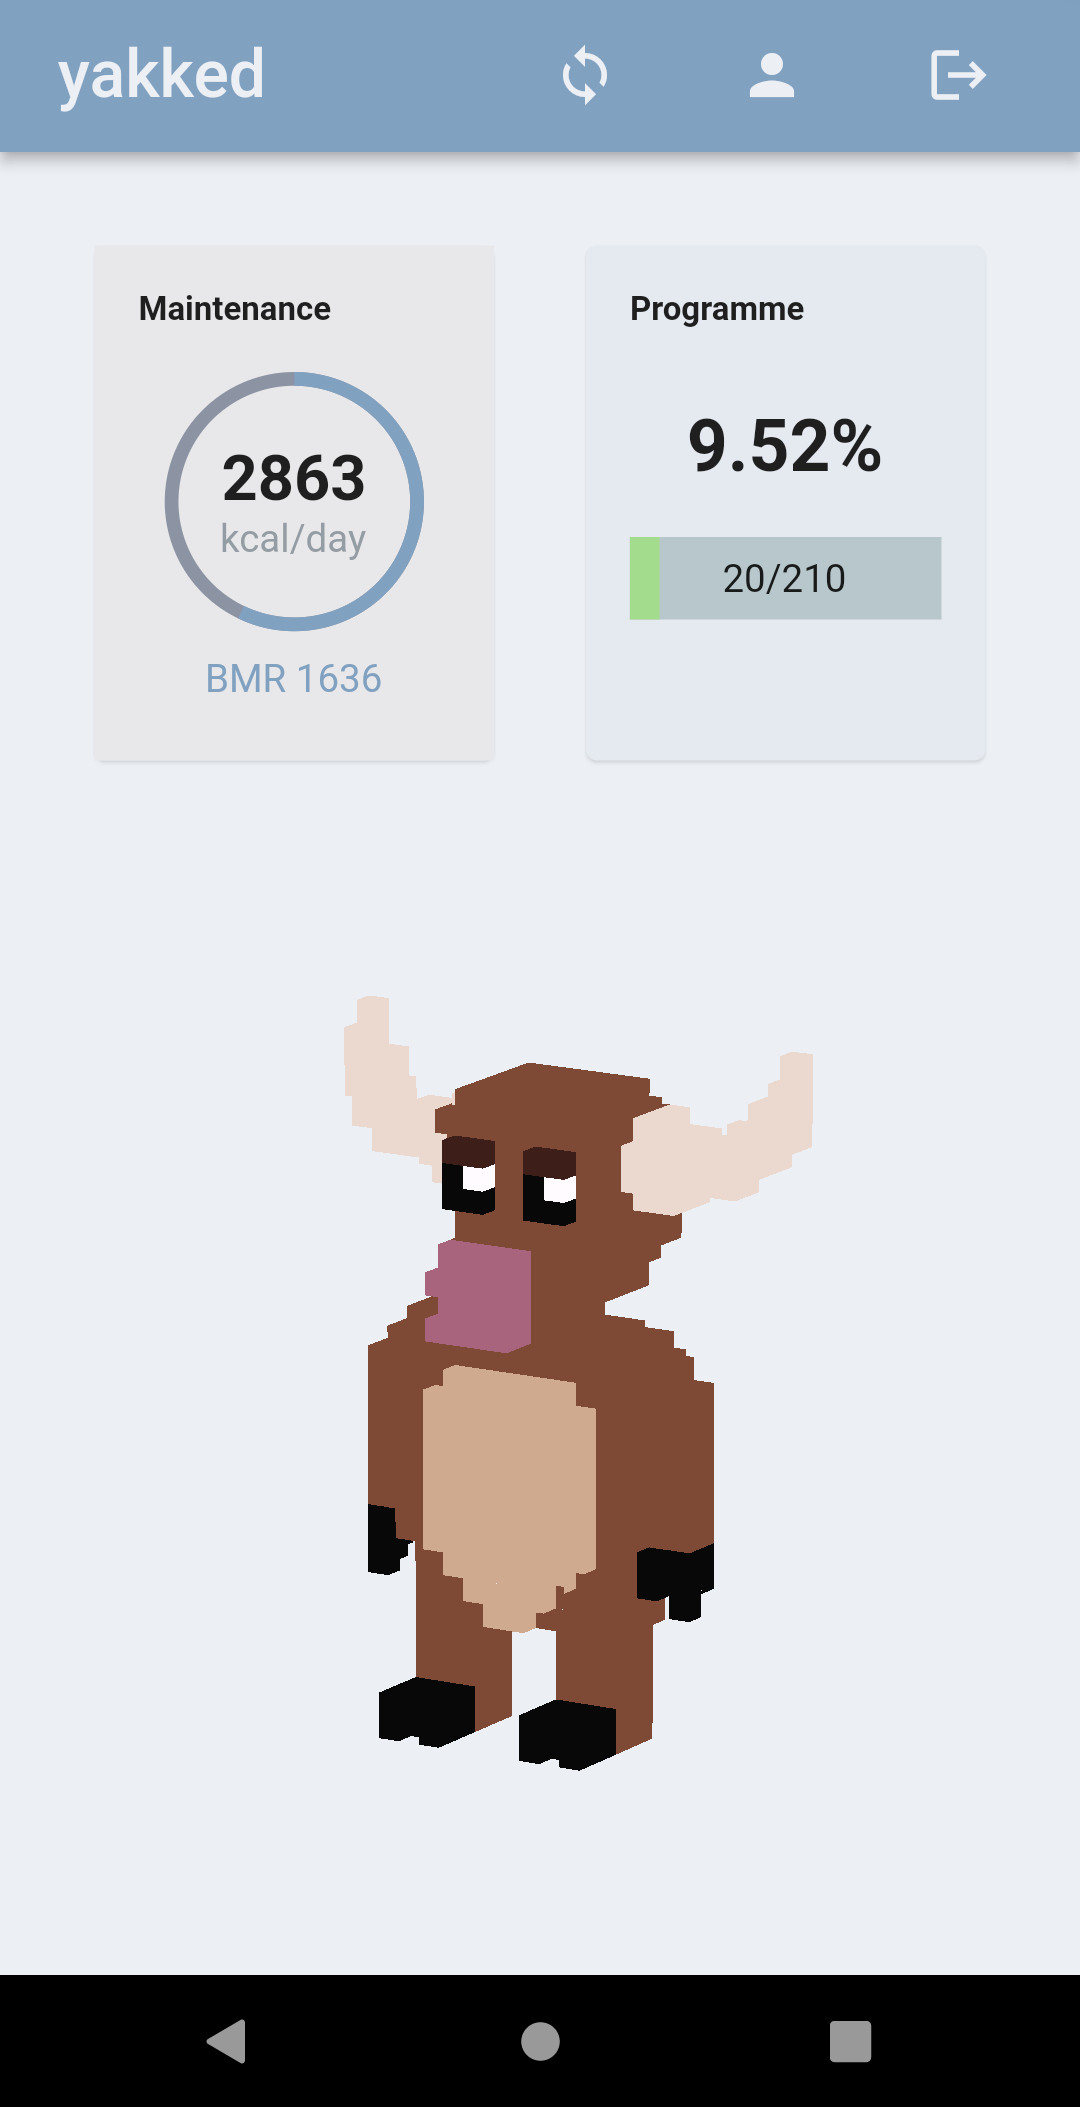
\includegraphics[width=\linewidth]{resume/imgs/yakked/mob1.png}
  \end{subfigure}
  \begin{subfigure}[b]{0.21\linewidth}
    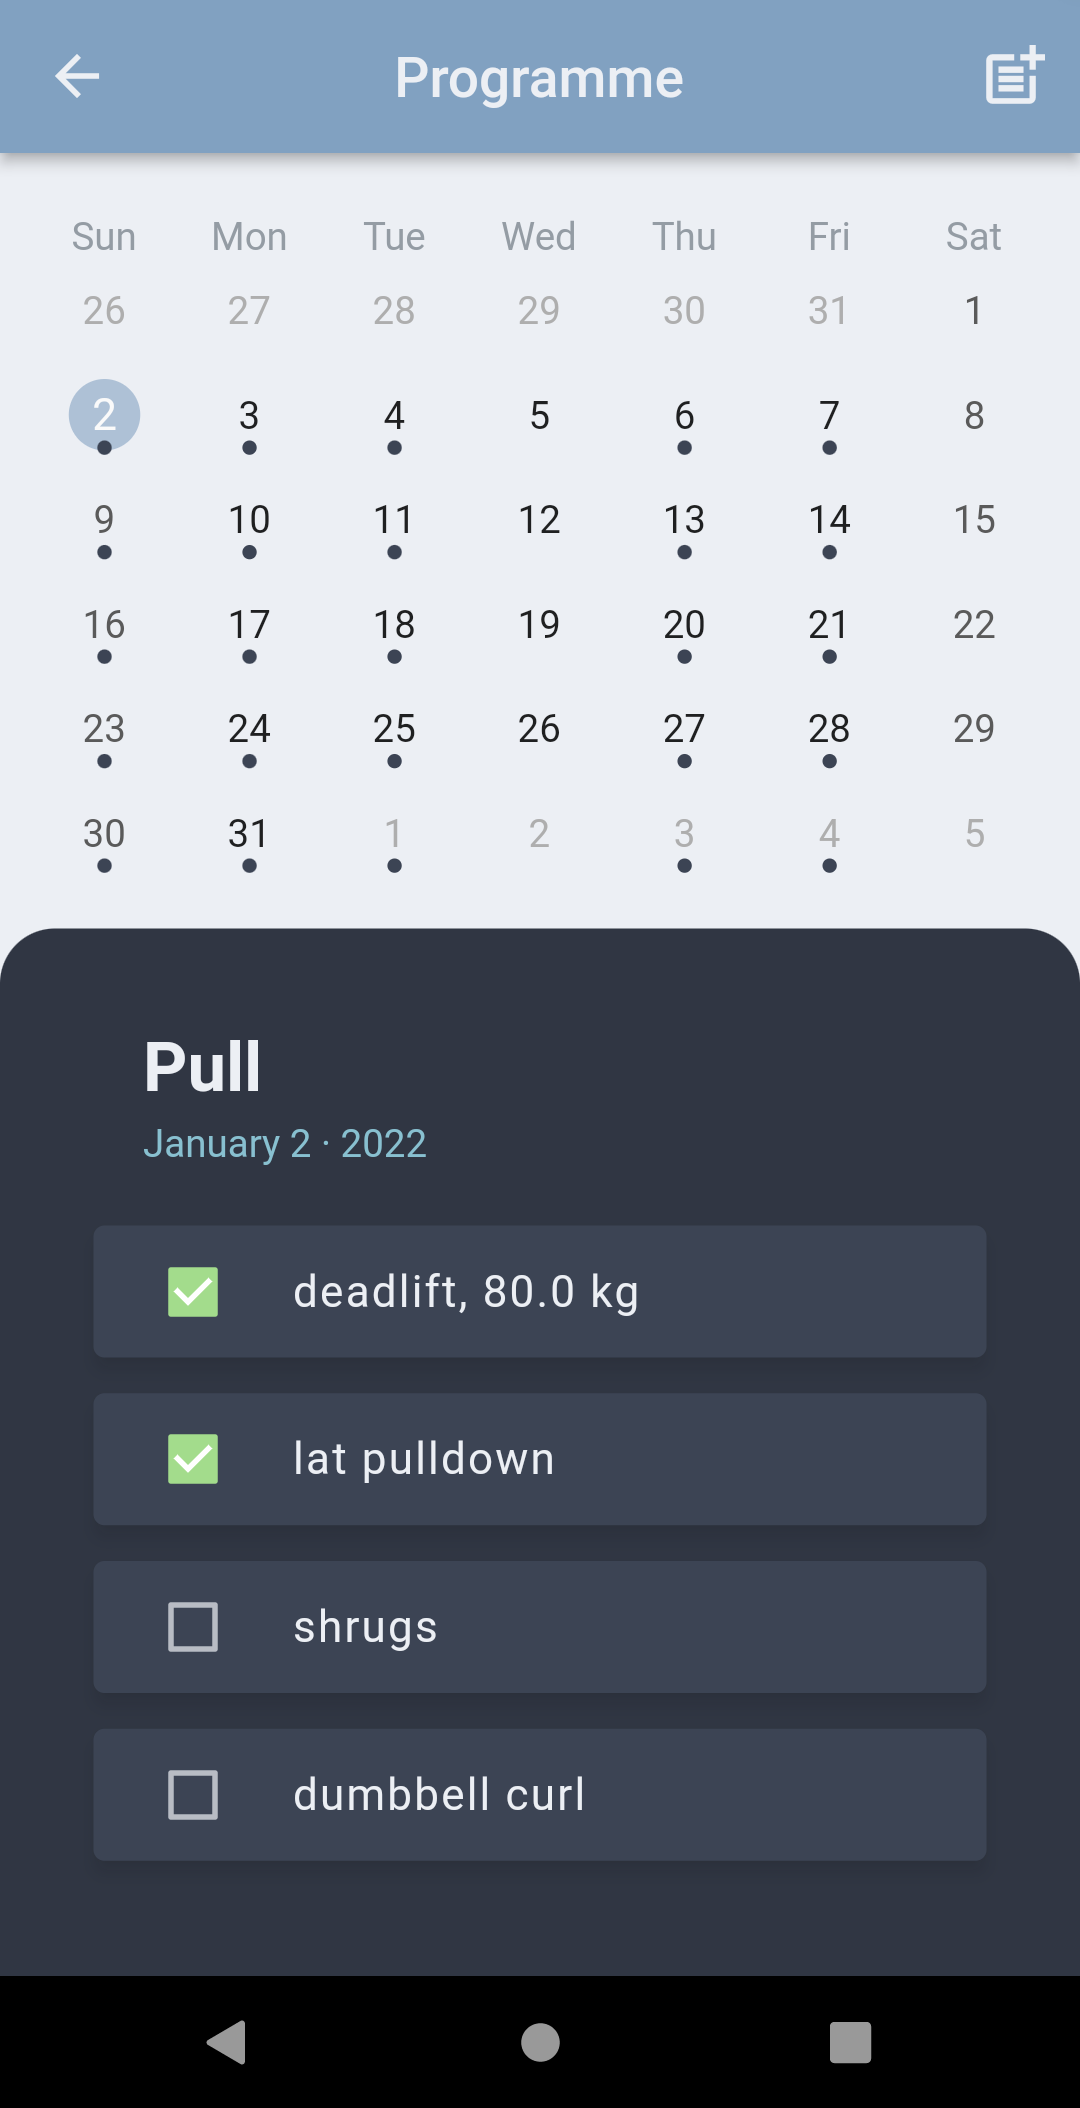
\includegraphics[width=\linewidth]{resume/imgs/yakked/mob2.png}
  \end{subfigure}
  \begin{subfigure}[b]{0.21\linewidth}
    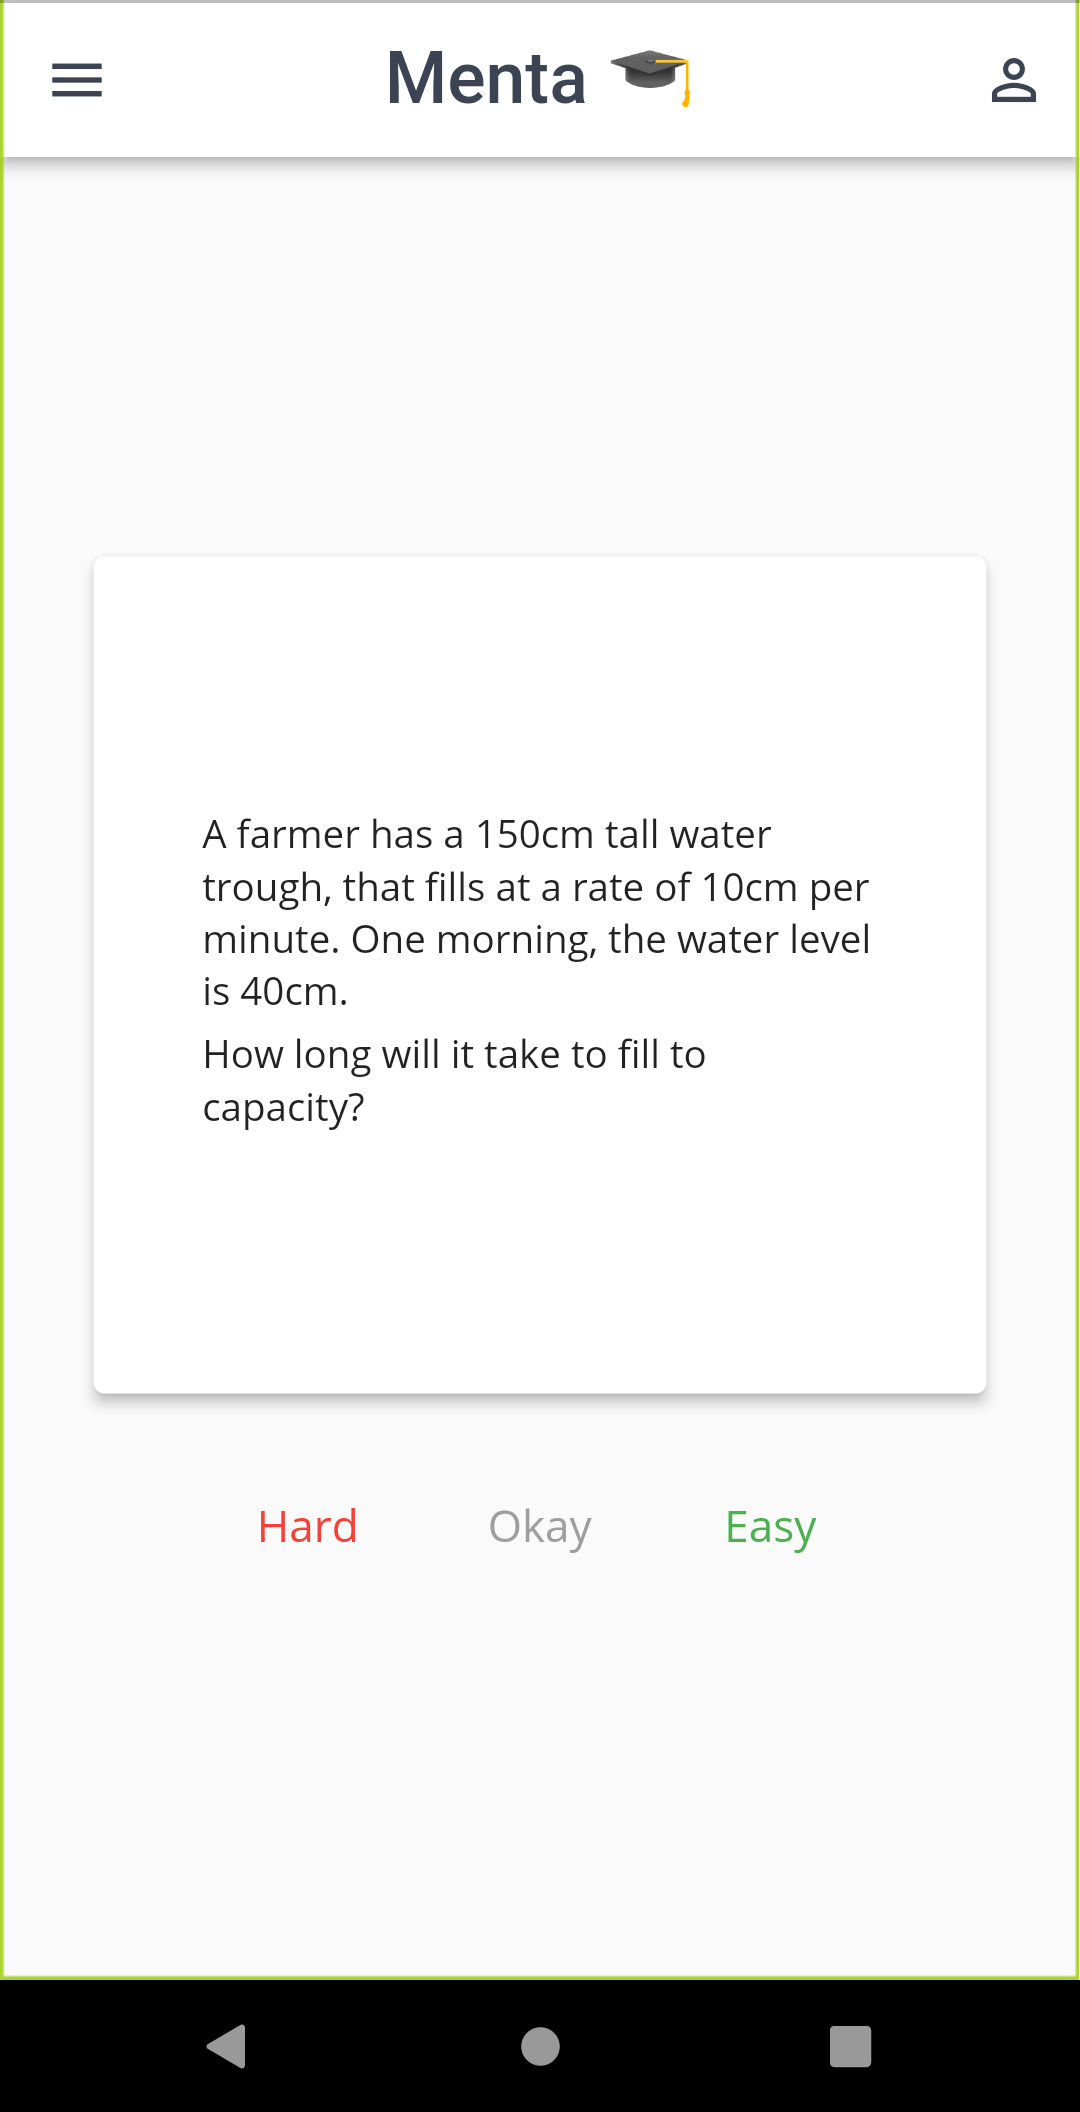
\includegraphics[width=\linewidth]{resume/imgs/menta/mob1.png}
  \end{subfigure}
  \begin{subfigure}[b]{0.21\linewidth}
    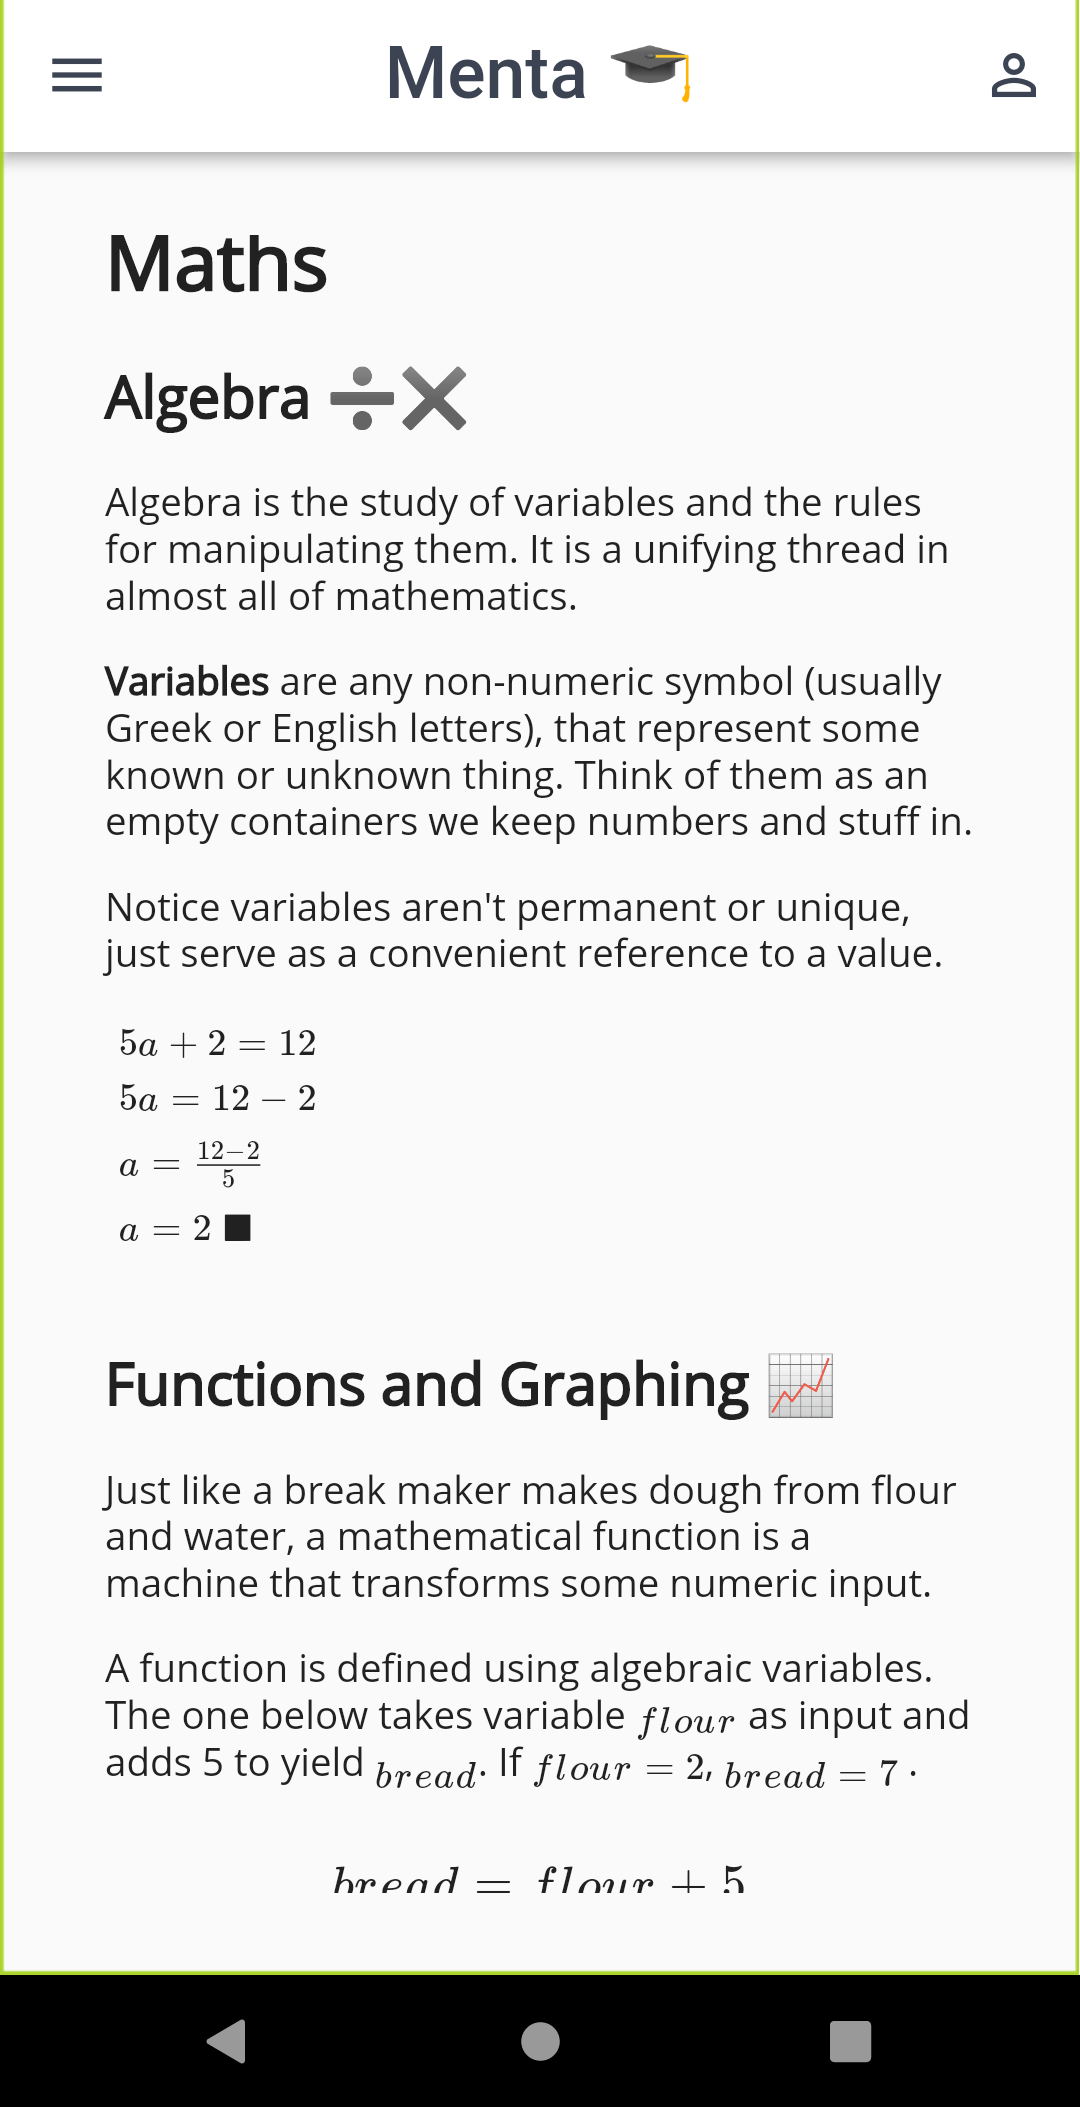
\includegraphics[width=\linewidth]{resume/imgs/menta/mob3.png}
  \end{subfigure}
  \caption{Flutter apps with Node and Golang backends}
  \label{fig:coffee}
\end{figure}

\begin{figure}[h!]
	\centering
	\includegraphics[width=0.84\textwidth]{resume/imgs/sirikit.png}
	\caption{Queen Sirikit Convention Centre "AnythingCanBreak" exhibit}
\end{figure}


%-------------------------------------------------------------------------------
\end{document}
